\chapter{Architecture and Memory}
\label{ch:architecture_and_memory}

The execution model associated with a high-level program does not mirror the actual underlying processor hardware. Instead of directly writing raw instructions for a CPU's fetch-decode-execute cycle, modern programming languages provide an abstraction layer. This layer relies on structured data, intermediate representations, and a runtime library to manage the execution environment. The high-level code we write is translated by the compiler into machine instructions, but its execution is supported by data structures managed behind the scenes. 

When a program runs, the operating system and the runtime library conspire to give it the illusion of being the sole user of the machine, with a vast, continuous memory space at its disposal. However, this virtual address space is not a single infinite void. It is carefully segmented to handle different types of data with different life cycles.

\begin{insightbox}
\textbf{The Illusion of Infinite Memory} \\
Languages often abstract away memory limits. A program requests memory, and the system complies. However, physical memory is finite. The operating system uses virtual memory and paging to extend available space, but bounds always exist. Recursion limits and out-of-memory errors are stark reminders of the physical hardware beneath the abstraction.
\end{insightbox}

\section{The True Beginning: Before and After \texttt{main}}
While we often consider the \texttt{main} function to be the starting point of our program, it is merely the user's entry point. Behind the scenes, the runtime library inserts a hidden startup function (often called \texttt{\_start} or \texttt{CRTmain}). This function prepares the memory layout, sets up the \texttt{argc} and \texttt{argv} parameters, and ultimately calls \texttt{main}. When \texttt{main} finishes, the runtime takes back control to properly dismantle the execution environment before handing control back to the operating system.

To understand how programs manage state, we must examine the internal layout of the program's address space. Typically, this space is divided into several areas:
\begin{itemize}
    \item \textbf{Executable Code:} The actual machine instructions.
    \item \textbf{Constants:} Immutable data, such as string literals (e.g., \texttt{"Hello, World"}), mapped as read-only.
    \item \textbf{Global Variables:} Variables that exist before the program starts and remain until termination, holding fixed addresses determined at compile time.
    \item \textbf{The Stack:} Used for managing function calls and local variables.
    \item \textbf{The Heap:} Used for dynamic memory allocation.
\end{itemize}

\begin{figure}[h]
    \centering
    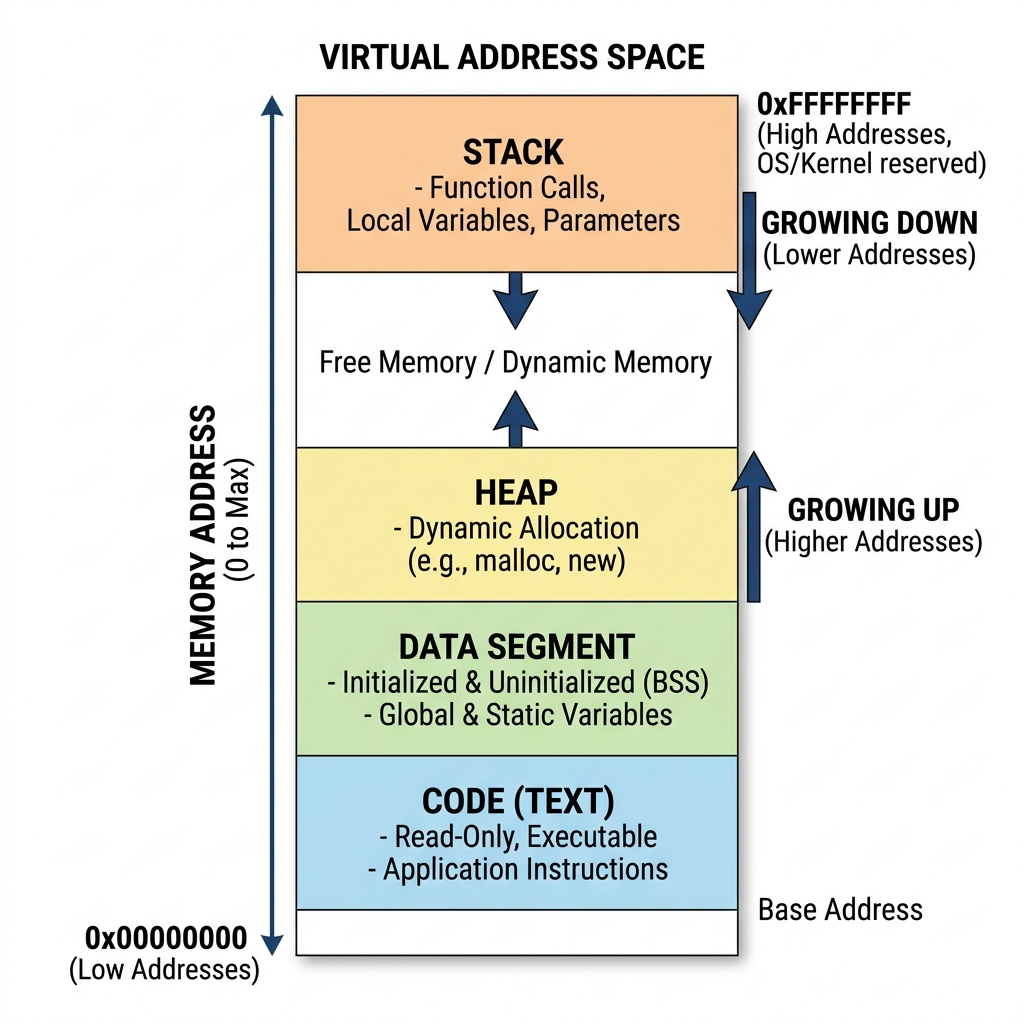
\includegraphics[width=0.5\textwidth]{images/memory_layout.png}
    \caption{Typical Memory Layout of a Process.}
    \label{fig:memory_layout}
\end{figure}

\begin{insightbox}
\textbf{Inspecting the Address Space} \\
On Linux or WSL2, you can directly inspect the segmented address space of a running process. Every process is assigned a Process ID (PID). By reading the virtual file \texttt{/proc/<PID>/maps}, you can see exactly which memory ranges are mapped to the Heap, the Stack, executable code, and shared libraries. Attempting to access an address outside these mapped ranges, or violating their access permissions (e.g., trying to write to the read-only constants area), immediately triggers a \texttt{Segmentation Fault}.
\end{insightbox}

The most critical distinction for a systems programmer is understanding how and when to use the Stack versus the Heap.

\section{The Stack: Automatic and Deterministic}

The Stack is a predefined block of memory provided by the operating system when the program starts. It is designed to manage the execution of functions, keeping track of where we are, what variables we have, and where we must return when a function completes.

\subsection{How the Stack Works}
Consider a simple function call. When \texttt{main} calls a function \texttt{f(v)}, several things must happen in a highly structured order:
\begin{enumerate}
    \item \textbf{Preparation:} Space is reserved for the return value of \texttt{f}.
    \item \textbf{Parameters:} The arguments (e.g., \texttt{v}) are copied into the stack so \texttt{f} can access them.
    \item \textbf{Return Address:} The address of the next instruction in \texttt{main} is pushed onto the stack so execution can resume correctly.
    \item \textbf{Local Variables:} As \texttt{f} executes, any local variables it declares are pushed onto the top of the stack.
\end{enumerate}

Beyond managing function variables, the Stack in languages like C++ also holds crucial metadata for structured exception handling. If a critical error occurs (such as a full disk or an interrupted network connection), the program uses this information to "unwind" the stack, safely skipping remaining operations and jumping to an appropriate error handler.

\begin{lstlisting}[language=C++]
int f(int a) {
    int i = 5;      // Local variable pushed onto the stack
    return a + i;   // Value is computed and placed in the return slot
}

int main() {
    int v = 9;         // Local variable in main's stack frame
    int result = f(v); // Triggers a new stack frame
    return 0;
}
\end{lstlisting}

\textbf{Deep Memory Model Analysis:}
In the snippet above, \texttt{v} is allocated on \texttt{main}'s stack frame. When \texttt{f(v)} is called, the value of \texttt{v} is copied into the parameter \texttt{a} on \texttt{f}'s new stack frame. The local variable \texttt{i} is also stack-allocated within \texttt{f}'s frame. Because these are purely value types (\texttt{int}), no heap allocation occurs. When \texttt{f} returns, its entire stack frame---including \texttt{a} and \texttt{i}---"evaporates", returning the computed value to \texttt{main}'s pre-allocated return slot.

When \texttt{f} finishes, it executes a \texttt{return}. The result is deposited in the reserved space, and the stack pointer is forcefully pulled back to its position before \texttt{f} was called. All the local variables and parameters of \texttt{f} instantly "evaporate." The memory is not physically erased, but it is released and will be overwritten by the next function call. 

\begin{notebox}
\textbf{The AirBnB Analogy} \\
Think of the stack like an AirBnB rental. You arrive, use the space for your stay, and then leave. The next guest will occupy the exact same room and overwrite whatever "mess" you left behind. This is why local variables in C/C++ contain unpredictable garbage values if not explicitly initialized—they simply hold the leftover data from previous stack frames!
\end{notebox}

\subsection{Trade-offs of the Stack}
The Stack is incredibly efficient. Allocation and deallocation are instantaneous, requiring only the adjustment of a single pointer. It guarantees perfect deterministic lifetimes: a variable's life is strictly bound to its lexical scope. Furthermore, because it operates sequentially in contiguous memory, it is highly cache-friendly.

\textbf{When and Why to Use It:} Prefer stack allocation whenever possible. It provides zero-cost automatic memory management and excellent cache locality. Use it for local variables, small fixed-size arrays, and values that do not need to outlive their declaring function scope.

However, the Stack is fundamentally limited. First, its size is fixed (often around a megabyte). Deep recursion will exhaust this space, resulting in a Stack Overflow. Second, the strict life cycle means a function cannot create data on the stack and pass it upwards to live longer than the function itself. 

\section{The Heap: Dynamic and Flexible}

When a program needs memory that outlives the function that created it, or requires a dynamically determined size that is too large for the stack, it must turn to the Heap. The Heap is a vast, unorganized area of memory managed by the OS and the runtime library. 

Unlike the Stack, memory on the Heap is not given out automatically. You must explicitly request it using an allocation function (e.g., \texttt{malloc} in C, or \texttt{new} in C++). The runtime searches for an available chunk of memory, marks it as reserved, and returns a \textit{pointer} to its starting address.

\begin{lstlisting}[language=C++]
int* create_array(int size) {
    if (size > 0) {
        // Requesting dynamic memory on the Heap.
        // C equivalent: int* buffer = malloc(size * sizeof(int));
        int* buffer = new int[size]; 
        
        // Ownership of this memory is passed back to the caller.
        // The data will survive even after create_array returns!
        return buffer; 
    }
    return nullptr;
}

int main() {
    int* my_array = create_array(2);
    
    if (my_array != nullptr) {
        // ... use my_array across different functions ...
        
        // When done, we MUST explicitly release it.
        // C equivalent: free(my_array);
        delete[] my_array; 
    }
    return 0;
}
\end{lstlisting}

\textbf{Deep Memory Model Analysis:}
Here, \texttt{create\_array} allocates memory on the heap via \texttt{new int[size]}. The pointer \texttt{buffer} itself is stored on the stack, but the array it points to resides on the heap. Ownership of this heap allocation is implicitly transferred back to \texttt{main} when the pointer is returned. In \texttt{main}, \texttt{my\_array} holds this pointer. Because C/C++ does not automatically track or enforce ownership semantics, it is strictly up to the programmer to ensure \texttt{delete[] my\_array} is called exactly once. Failure to do so leads to a memory leak.

\subsection{The Burden of Manual Management}
\textbf{When and Why to Use It:} Use heap allocation when the size of the data is unknown at compile time, when the data is too large to fit safely on the stack (risking a Stack Overflow), or when the data must outlive the function that created it.

The great flexibility of the Heap comes with a heavy responsibility. The compiler and runtime do not track when you stop using a dynamically allocated block. It is entirely up to the programmer to return the "key" to the runtime by calling \texttt{free()} or \texttt{delete}. 

If you forget to release the memory, it remains marked as "in use." If this happens repeatedly, the program will consume more and more memory until the OS refuses to provide any more, causing an application crash. This phenomenon is known as a \textbf{memory leak}.

\subsection{Beyond the Stack and Heap: The Message Queue}
While the Stack and Heap form the core of C and C++ memory management, other execution environments (such as JavaScript or TypeScript) rely on a third fundamental structure: the \textbf{Message Queue}. This queue operates on a First-In, First-Out (FIFO) basis, intercepting asynchronous events like mouse clicks, network responses, and timers, dispatching them to the execution thread when it is free.

\section{The Danger of Pointers}

Pointers are the only way to interact with the Heap, yet they are intrinsically ambiguous and dangerous. A pointer is simply a numerical memory address (e.g., \texttt{0x3B7F}), but the language provides almost no metadata about it.

\begin{examprioritybox}
\textbf{The Ambiguity of Pointers in C/C++} \\
When a C++ programmer looks at an \texttt{int* ptr}, they cannot answer fundamental questions:
\begin{itemize}
    \item \textbf{Validity:} Is the address valid? By convention, \texttt{0} is a null pointer, but if it is \texttt{0x3B7F}, it might point to a valid integer, or it might point to unowned garbage.
    \item \textbf{Ownership:} Am I responsible for freeing this pointer, or is another function managing it?
    \item \textbf{Multiplicity:} Is this pointer an array of integers, or just a single integer?
    \item \textbf{Lifetime:} How long is this memory guaranteed to remain valid? The professor often compares this to a carton of milk lacking an expiration date.
\end{itemize}
\textbf{Common Pitfall:} Assuming a non-null pointer is safe to dereference or free without verifying ownership. \\
\textbf{Expected Mastery Level:} High. You must explicitly recall these four missing metadata elements, as they are central to understanding why Rust's type system is designed the way it is.
\end{examprioritybox}

To understand the lifetime ambiguity, consider an analogy: when you buy a carton of milk at the supermarket, it comes with a clear expiration date. You know exactly when it will go bad. Pointers, unfortunately, do not have an expiration date stamped on them. If you save a pointer to be used later, the language provides no built-in mechanism to check if the underlying memory has been released by another part of the program in the meantime. 

Consider the notorious \textbf{Use-After-Free} bug. Because pointers are immaterial copies of addresses, releasing the memory does not destroy the pointer variables that hold that address.

\begin{lstlisting}[language=C++]
int* ptr = new int(42);
delete ptr; // Memory is returned to the OS.

// 'ptr' is now a Dangling Pointer. 
// It still holds the address, but we no longer own the memory!
*ptr = 100; // Undefined Behavior! Writing to unowned memory.
\end{lstlisting}

To avoid this, a disciplined programmer must manually track pointer lifecycles, which is notoriously difficult in large, complex codebases.

\section{Garbage Collection vs. Rust}

To solve the pointer crisis, many modern languages (Java, Python, C\#) abandoned manual memory management entirely, introducing a \textbf{Garbage Collector (GC)}.

In Java, elementary types (like \texttt{int}) live on the stack with value semantics, but objects live on the heap with reference semantics.

\begin{lstlisting}[language=Java]
// Java GC Example
int i = 5; // Value on the stack

// Semantic of reference
String s = "ciao mamma"; // Allocated on the Heap
ArrayList<Integer> list = new ArrayList<>(); // Allocated on the Heap

// Notice: No explicit free() or delete! 
// The Garbage Collector will eventually clean them up.
\end{lstlisting}

With a GC, the programmer never calls \texttt{free()}. Instead, the runtime periodically pauses the program to scan the heap, look for objects that no longer have any active pointers referencing them, and reclaims their memory. The most renowned algorithms used for this task belong to the \textbf{Mark and Sweep} family, often coupled with \textbf{Reference Counting} strategies. 

\begin{examprioritybox}
\textbf{The Cost of Garbage Collection} \\
While GCs eliminate memory leaks and use-after-free bugs, they introduce non-deterministic pauses ("Stop The World" events). When the GC runs, the execution of the main program halts. As emphasized in lectures, this pause can last seconds, which for a CPU doing a billion operations per second is an eternity. \\
\textbf{Common Pitfall:} Believing GC solves all memory issues without side effects. In real-time systems (e.g., medical devices, aerospace), this lack of predictability is entirely unacceptable. \\
\textbf{Expected Mastery Level:} High. Be prepared to contrast GC latency with Rust's compile-time memory management.
\end{examprioritybox}

\subsection{The Rust Paradigm}
Rust enters the landscape with a bold proposition: \textit{Safety without Garbage Collection}. Systems programmers want the determinism and extreme performance of C/C++, but without the undefined behavior and pointer bugs. 

Rust achieves this by embedding memory management rules directly into its type system. Instead of having a single, ambiguous \texttt{int*} pointer, Rust distinguishes between different types of ownership and borrowing. By forcing the programmer to explicitly state who owns the memory and how long it lives, the Rust compiler can insert the necessary \texttt{free} calls automatically at compile time, eliminating both the GC overhead and manual memory bugs.

\subsection*{Exam Relevance and Recurrence}
\textbf{Score:} Very High \\
\textbf{Notes:} The fundamental differences between stack and heap, and the intrinsic ambiguities of C/C++ pointers, frequently appear in exams. The "Stop The World" problem of Garbage Collection and how Rust fixes this via ownership rules is a recurring short-essay question.

\section{Domande ed Esercizi da Esami Passati}

\begin{exambox}
\textbf{Domanda 1:} Si illustrino le differenze tra stack e heap. Insieme alle differenze, indicare per i seguenti costrutti Rust, in modo dettagliato, dove si trovano i dati che li compongono: \texttt{Box<[T]>}, \texttt{RefCell<T>} e \texttt{\&[T]}.
\end{exambox}
\textbf{Soluzione basata sul capitolo:} 
Lo \textbf{Stack} è una memoria efficiente e deterministica fornita dal sistema operativo, utilizzata per la gestione delle chiamate a funzione e delle variabili locali. L'allocazione e deallocazione avvengono spostando un singolo puntatore (stack pointer) in modo quasi istantaneo. I dati hanno un ciclo di vita limitato allo scope della funzione in cui sono definiti e la dimensione totale dello stack è fissa.
L'\textbf{Heap} è un'area di memoria vasta e non organizzata, utilizzata per l'allocazione dinamica, essenziale quando la dimensione dei dati non è nota a compile time o quando i dati devono sopravvivere alla funzione che li ha creati. L'heap richiede un'allocazione e deallocazione esplicita (rischio di memory leak e dangling pointer in assenza di Garbage Collection o del type system di Rust).
\textit{Nota sui costrutti Rust:} Il capitolo si focalizza sui principi generali della memoria in C/C++ e sul superamento del Garbage Collector in Rust, ma non dettaglia l'implementazione in memoria di \texttt{Box}, \texttt{RefCell} o \texttt{\&[T]}. In base ai concetti del capitolo, si deduce unicamente che eventuali puntatori alle risorse risiedono sullo stack locale, mentre i dati gestiti dinamicamente risiedono nell'heap.

\begin{exambox}
\textbf{Domanda 2:} Si definiscano le principali aree di memoria associate ad un eseguibile e si mostri, attraverso opportuni esempi di codice, in quale situazione ciascuna di esse viene utilizzata.
\end{exambox}
\textbf{Soluzione basata sul capitolo:} 
Lo spazio di indirizzamento virtuale di un processo è diviso nelle seguenti aree principali:
\begin{itemize}
    \item \textbf{Executable Code:} contiene le istruzioni macchina da eseguire.
    \item \textbf{Constants:} area a sola lettura per i dati immutabili, ad esempio i letterali stringa (es. \texttt{"Hello, World"}).
    \item \textbf{Global Variables:} variabili i cui indirizzi sono determinati a tempo di compilazione e persistono per tutta la durata del programma.
    \item \textbf{Stack:} utilizzato per la gestione automatica delle chiamate a funzione e delle variabili locali. \textit{Esempio:} In \texttt{int f(int a) \{ int i = 5; return a + i; \}}, le variabili \texttt{a} e \texttt{i} sono collocate sullo stack del rispettivo frame.
    \item \textbf{Heap:} area usata per l'allocazione dinamica. \textit{Esempio:} In \texttt{int* buffer = new int[size];}, l'array la cui dimensione è calcolata a runtime viene allocato nello heap, mentre il puntatore \texttt{buffer} che ne mantiene l'indirizzo si trova nello stack.
\end{itemize}

\begin{exambox}
\textbf{Domanda 3:} Si considerino le seguenti strutture dati e rispettive porzioni di codice. Per ciascuna di esse si indichi la dimensione di memoria allocata nello stack e nello heap, ipotizzando un’architettura a 64 bit.
\begin{verbatim}
let boxed: Box<[u32]> = vec![10, 20, 30, 40,
\end{verbatim}
\end{exambox}
\textbf{Soluzione basata sul capitolo:}
Il Capitolo 2 non include le nozioni per calcolare la dimensione in byte per architetture a 64 bit o il dettaglio dei tipi \texttt{Box} e \texttt{vec!}. Applicando esclusivamente la teoria del capitolo: la variabile locale \texttt{boxed} occupa memoria nello \textbf{stack} (poiché conterrà il puntatore o il descrittore del dato), mentre l'allocazione dinamica dei valori forniti a runtime avverrà nell'\textbf{heap}.

\begin{exambox}
\textbf{Domanda 4:} Sia data la struttura \texttt{LinkedList<T>} definita come:
\begin{verbatim}
pub struct LinkedList<'a, T> { 
    pub val: Option<T>, 
    pub next: Option<&'a Box<LinkedList<'a, T>>>, 
}
\end{verbatim}
Si definisca l’occupazione di memora di un elemento della lista e si indichi come sia possibile definire il fine lista.
\end{exambox}
\textbf{Soluzione basata sul capitolo:}
Il testo affronta il layout di memoria generico (Code, Data, Stack, Heap) e i concetti di ownership senza calcolare il footprint in memoria di strutture Rust specifiche. Pertanto, l'occupazione in memoria dell'elemento non è ricavabile. Il fine lista, basandosi sul parallelismo con l'assenza di riferimenti validi discussa per i puntatori nulli (es. \texttt{0} in C/C++), si modellerà in Rust indicando la non presenza di un puntatore successivo (ovvero con la variante \texttt{None} dell'\texttt{Option}, anche se non descritto esplicitamente nel capitolo).

\begin{exambox}
\textbf{Domanda 5:} Data la struttura dati definita come
\begin{verbatim}
struct Data { Element: AsVector, next: Rc<Data> }
enum AsVector { AsVector(Box::<Rc<i32>>), None }
\end{verbatim}
Indicare l’occupazione di memoria di un singolo elemento in termini di: 1. numero di byte complessivi (caso peggiore, architettura a 64 bit) e 2. posizionamento dei vari byte in memoria (stack, heap, ecc.).
\end{exambox}
\textbf{Soluzione basata sul capitolo:}
\begin{enumerate}
    \item \textbf{Numero di byte:} Non calcolabile, poiché il capitolo non specifica la grandezza in byte di puntatori, \texttt{enum}, \texttt{Box} o \texttt{Rc}.
    \item \textbf{Posizionamento in memoria:} Sulla base della logica introdotta nel testo, l'elemento allocato all'interno di una funzione occuperà memoria sullo \textbf{Stack} per le sue componenti di base (come per i puntatori \texttt{int* ptr} e le variabili locali). Tuttavia, la memoria sottostante effettivamente incapsulata e gestita dinamicamente da tipi come \texttt{Box} o \texttt{Rc} risiederà nell'\textbf{Heap}.
\end{enumerate}
